%!TEX root = ../Dokumentation.tex


\section{Entwicklung eines User-Client}

\subsection{Vorbereitung und Layoutentwicklung}
Im finalen Meilenstein des Projektes, steht die Entwicklung eines grafischen Userinterface im Mittelpunkt, der die Funktionalität des Systems repräsentiert. Die Applikation soll die entsprechende Verbindung zum Server aufbauen und den Datenaustausch ermöglichen. \\

Vor der praktischen Umsetzung mit Java Swing, wurde ein mögliches Konzeptlayout erstellt und entsprechende Alternativen ausprobiert.Hierbei handelt es sich um erste Ideen wie die Anwendung aufgebaut sein kann und welche Elemente benötigt werden.
Da in der letztendlichen Umsetzung aber hauptsächlich die Funktionalität im Mittelpunkt steht, wurde speziell darauf geachtet, dass alle Funktionalitäten in einem logischen Kontext eingebunden werden und anwendbar sind. Auf genaue Designkonzepte zum optimalen Aufbau wurde hierbei verzichtet, da sie im entsprechenden Projektkontext nicht an erster Stelle stehen sollten. In einem größer angelegten Projekt sollte hierbei eine intensivere Auseinandersetzung folgen mit entsprechender Validierung und Testdurchläufe. \\

Die Applikation soll mit einer Startseite (Abb. 3.3a) beginnen, von der aus der Anwender die Möglichkeit hat sich zu identifizieren. Entweder er meldet sich mit bereits vorhandenen Daten an oder er registriert sich als neuer Benutzer.
Sind bereits Accountdaten vorhanden, so folgt eine Eingabe des Usernamen und des Passworts (Abb. 3.3b). Sollte der User eine der beiden Informationen vergessen haben, so besteht die Option \textit{Passwort/Username vergessen?}, wobei die funktionale Implementierung nicht stattfinden wird und dies eher als Platzhalter dient. Nach Eingabe der Daten und Prüfung auf Korrektheit, wird zur \textit{Homeseite} weitergeleitet, die als Hauptseite dient und von der aus die verschiedenen Funktionen angesteuert werden.

\begin{figure}[h!]
\centering
\hfill %
\subfloat[Startseite \label{pic:startseite}]{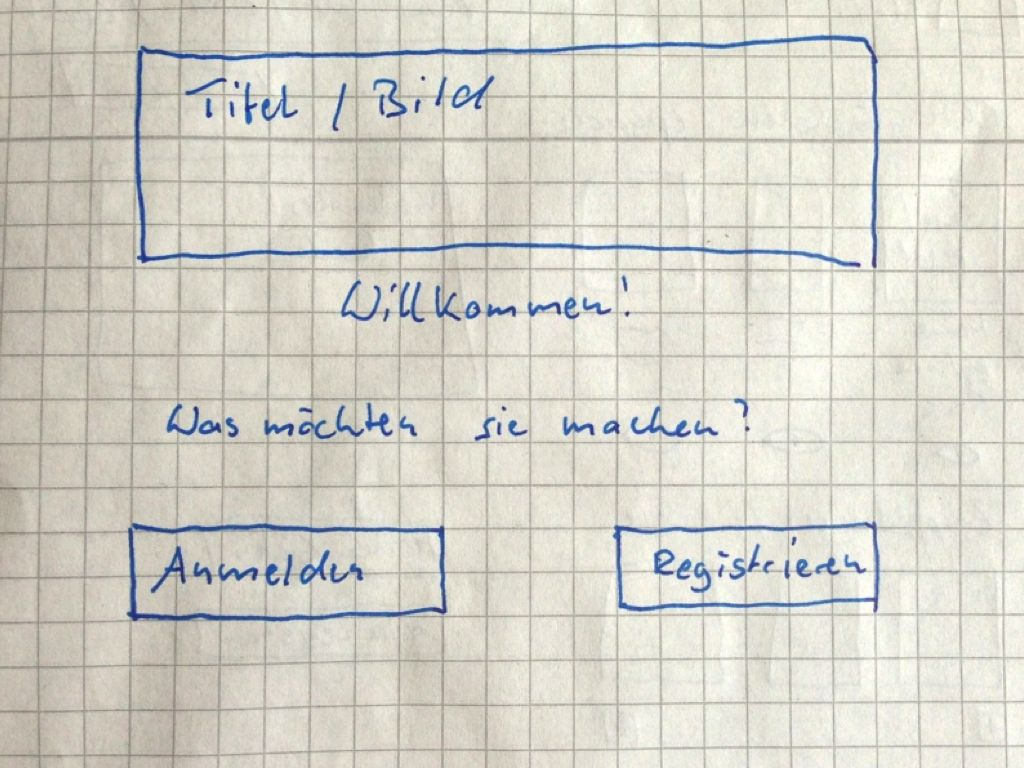
\includegraphics[width=.5\textwidth]{../images/dokulayout/startseite.jpg}}
\hfill % alternativ auch \hspace{1cm} für genaue Angaben
\subfloat[Einloggen \label{pic:anmelden}]{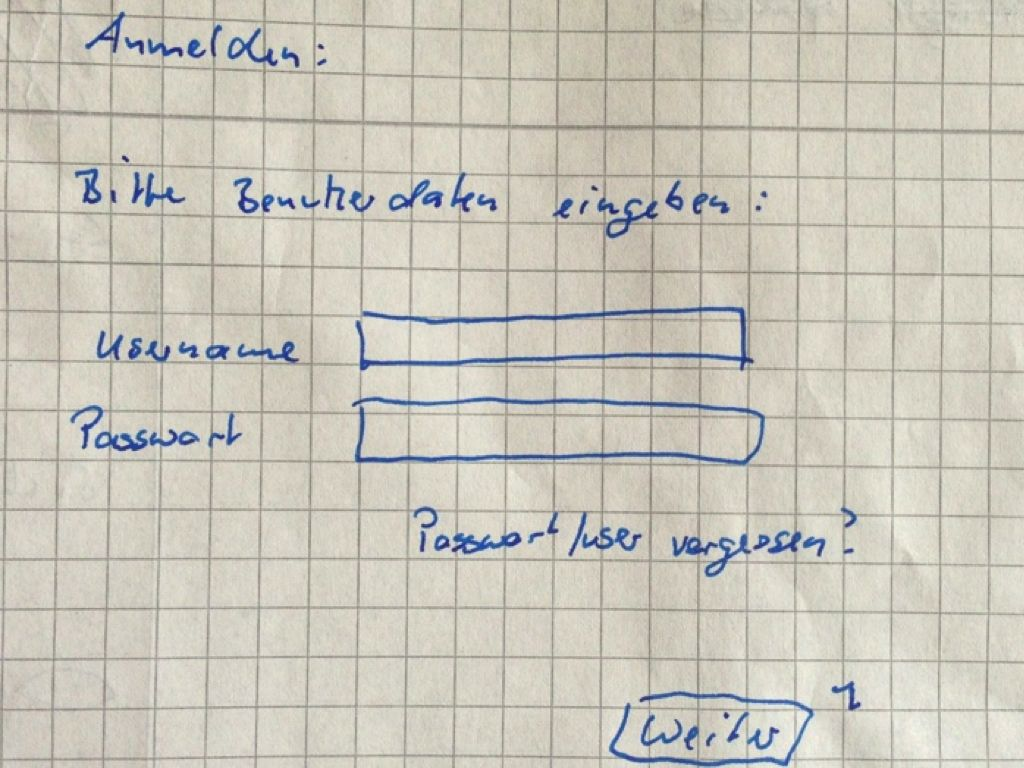
\includegraphics[width=.5\textwidth]{../images/dokulayout/anmelden.jpg}}
\hfill %
\caption{GUI Layout Skizzen: Startauswahl und Einloggen }
\label{gui-skizzen-start-login}
\end{figure}




\newpage

Entscheidet man sich für die Auswahl \textit{Registrieren} wird ein neuer Account angelegt. Auf der ersten Seite (Abb. 3.4a) werden die Grundinformationen eingegeben, wobei hier nur Username und Passwort und Name notwendig sind und die zusätzlichen Informationen jederzeit ergänzt werden können. Nach Eingabe und Kontrolle folgt der zweite Teil der Registrierung, die Auswahl der Genreprioritäten (Abb. 3.4b). Da der Serientracker die Option anbietet, Informationen zu Serien eines bestimtmen Genres zu erhalten, dient dieser Schritt dazu bestimmte Genres zu abonnieren. Auch hier soll die Auswahl später geändert werden können.\\

\begin{figure}[h!]
\centering
\hfill
\subfloat[Registrieren \label{pic:registrieren}]{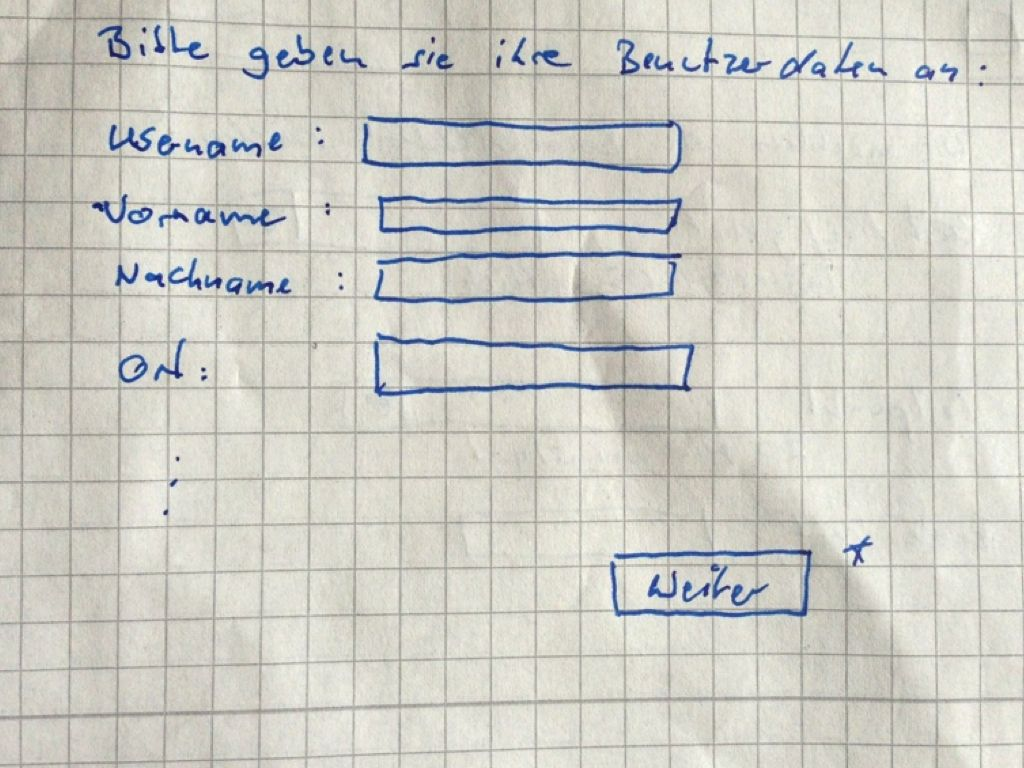
\includegraphics[width=.5\textwidth]{../images/dokulayout/registrieren.jpg}}
\hfill % alternativ auch \hspace{1cm} für genaue Angaben
\subfloat[Prioritäten \label{pic:prioritaeten}]{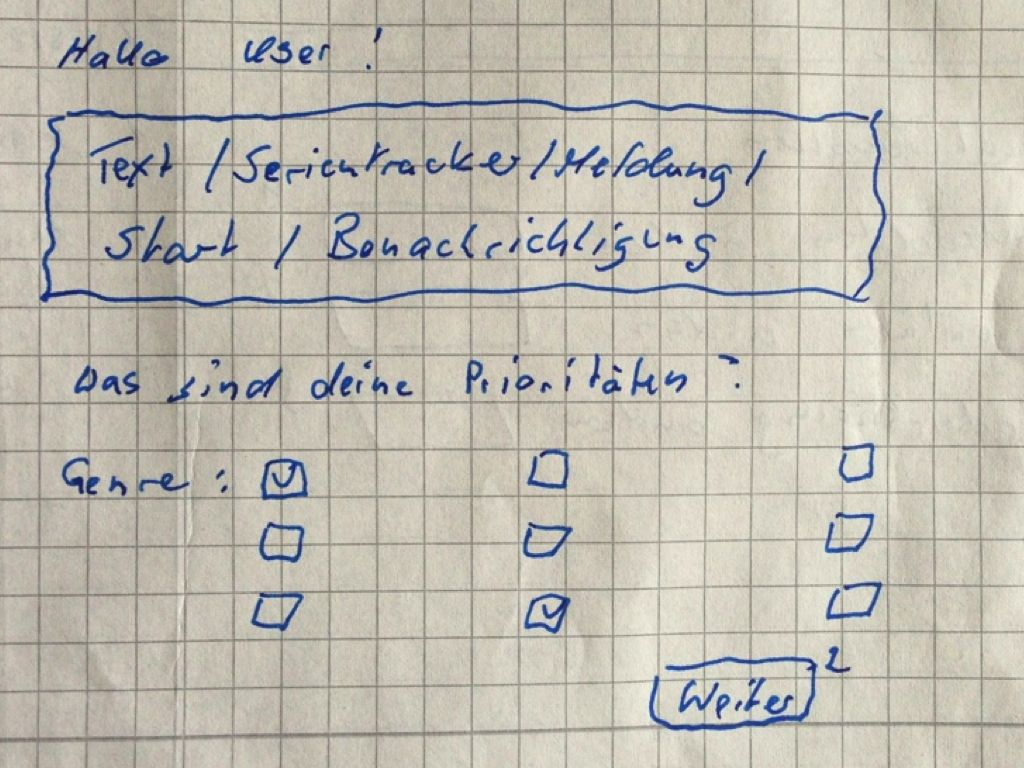
\includegraphics[width=.5\textwidth]{../images/dokulayout/prioritaeten.jpg}}
\hfill %
\caption{GUI Layout Skizzen: Registrierung }
\label{gui-skizzen-registrierung}
\end{figure}

\vspace{0.2cm}

\begin{wrapfigure}{r}{0cm}
\centering
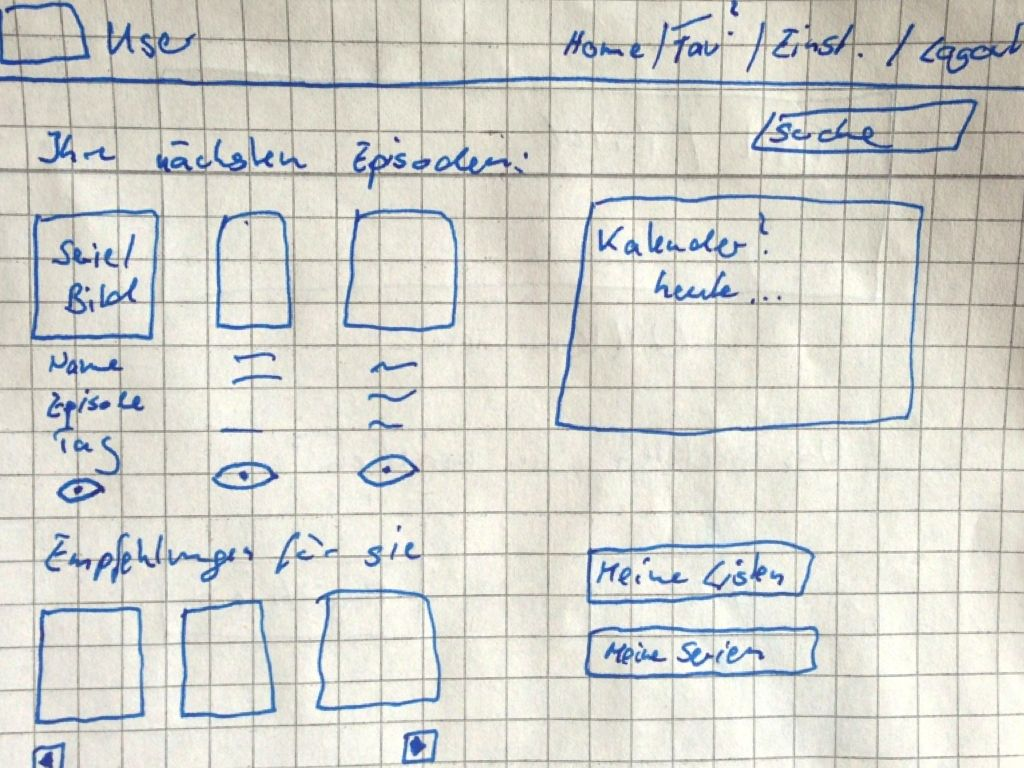
\includegraphics[width=.5\textwidth]{../images/dokulayout/home.jpg}
\caption{GUI Skizzen: Homeansicht}
\end{wrapfigure}

Nach erfolgreicher Identifizierung des Users folgt der Homebereich (Abb. 3.5). Dies ist der eigentliche Ausgangspunkt für alle Aktivitäten und dient als Benutzerzentrale. Am oberen Bereich findet sich eine statische Menüleiste, die sich in diesem Aufbau durch alle weiteren Bereiche zieht und jederzeit zugänglich ist. Information zum angemeldeten User und die Optionen \textit{Home}, \textit{Favoriten}, \textit{Einstellung}und\textit {Logout}. Home führt jederzeite zur Hauptübersicht, Einstellung ermöglicht entsprechende Möglichkeiten zur Accountverwaltung und Logout meldet den aktuellen Benutzer ab und führt wieder zur Anmeldung. Die Option Favoriten war als Verwaltung zu den angelegten Lieblingsgenre geplant, wurde aber in weiteren Entwürfen in die Einstellungen mit eingebunden, da bis auf eine einfache Auswahl kein größerer Nutzen für den User angeboten wird. Für den Fall das Adminrechte vorhanden sind, wurde in einem späteren Entwurf der zusätzliche Menüpunkt \textit{Hinzufügen} eingebunden. Dort lassen sich neue Serien, Staffeln, Episoden und Genrelisten anlegen. \\


Da im Mittelpunkt des Konzeptes die Benachrichtigung über neue Episoden steht, werden dem User bereits nach einloggen die wichtigsten Informationen präsentiert. Neben einer Suche, werden die Ausstrahlungszeitpunkte der nächsten Episoden angezeigt. Neben dieser Übersicht sollten zudem direkte Benachrichtigungen in Form von Pop-Ups stattfinden, weshalb diese Ansicht vorallem der Erinnerung und Verwaltung dient. Inwiefern eine Darstellung der heutigen Serien in Form eines Kalender realisierbar wäre ist zur Zeit der Konzipierung noch unklar, sollte aber eher als \textit{nice-to-have Feature} betrachtet werden.\\
Dazu gab es die Überlegung Serienempfehlung zu geben, basiernd auf abonnierten Genres. Buttons zu \textit{Meine Serien} und \textit{Meine Listen} führen zu entsprechenden Unterkategoerien.
Meine Serien zeigt einer Auflistung der Serien über die man Benachrichtigungen erhalten möchte und die derzeit angeschaut werden. Meine Listen gibt einen Überblick über angelegte Listen zur Ordnung von Serien nach bestimmten Themen und bietet zudem die Möglichkeit eine neue Liste anzulegen. \\

\parskip 12pt
\parindent 0pt

Nach Auswahl einer bestimmten Serie werden vorhandene Information präsentiert. Allgemeine Informationen, eine Übersicht zu vorhandenen Staffeln und eine Darstellung der nächsten Episode die Ausgestrahlt wird und gegebenfalls die Episode die der Benuter zuletzt gesehen hat. Hierbei würde die Verwaltung mit Hilfe der Seen List stattfinden, wobei auch hier die letztendliche Umsetzung eher unwahrscheinlich ist.
Auf dieser Seite (Abb. 3.6a) kann die Serie einer bestimmten Liste hinzugefügt werden und wird damit abonniert. In einer weiteren Variante der Serienseite (Abb. 3.6b) handelt es sich um die Darstellung unter Adminrechte, wobei die \textit{Add to List} Option nun zum Editieren dieser Seite führt und auch neben den Serien eine entsprechende Editierfunktion eingeführt wird.

\begin{figure} [h!]
\centering
\hfill %
\subfloat[Serienseite User \label{pic:serie}]{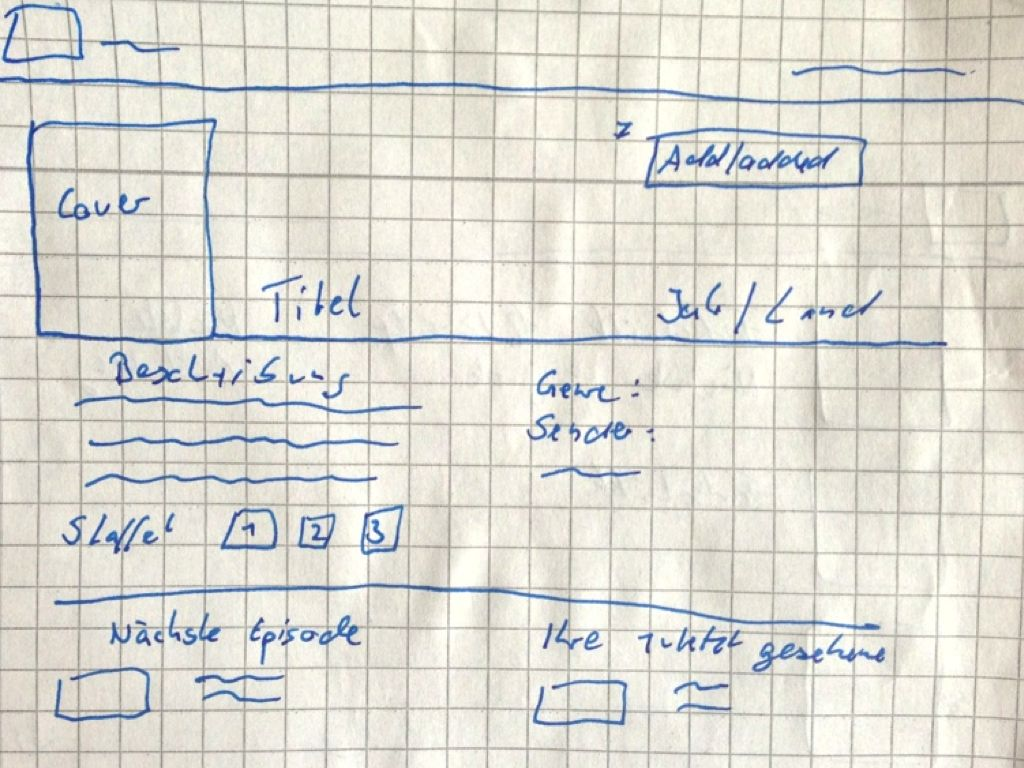
\includegraphics[width=.5\textwidth]{../images/dokulayout/serie.jpg}}
\hfill % alternativ auch \hspace{1cm} für genaue Angaben
\subfloat[Serienseite Admin \label{pic:serie2}]{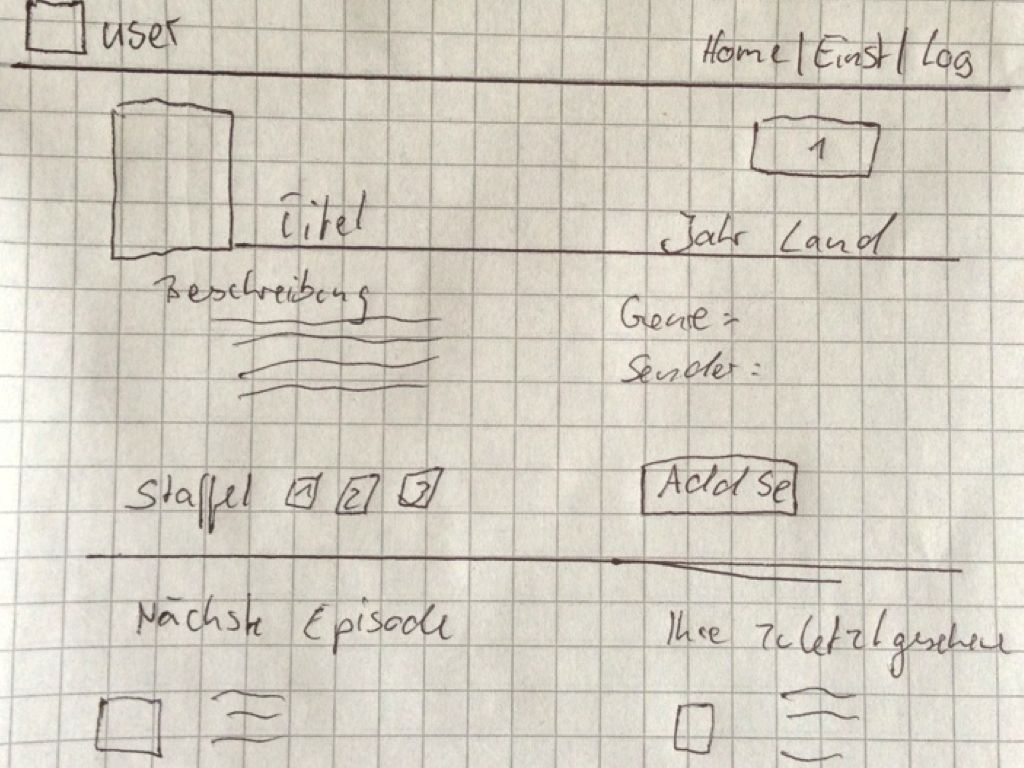
\includegraphics[width=.5\textwidth]{../images/dokulayout/serie2.jpg}}
\hfill %
\caption{GUI Layout Skizzen: Serienübersicht }
\label{gui-skizzen-serien}
\end{figure}


\newpage

Die jeweilige Seasonseite (Abb. 3.7a) zeigt eine Vorschau zu vorhandenen Episoden und bietet dem Admin erneut die \textit{Add Episode} Funktion (Abb. 3.7b). In welcher Form die Episoden aufgeführt werden ist zu diesem Zeitpunkt noch nicht festgelegt und wird bei entsprechender Umsetzung entschieden. Wird eine neue Episode angelegt (Abb. 3.7b) wird entsprechende Serie und Staffel referenziert und die einzelnrn Informationen eingegeben.\\
\begin{figure} [h!]
\centering
\hfill %
\subfloat[Seasonseite \label{pic:staffel}]{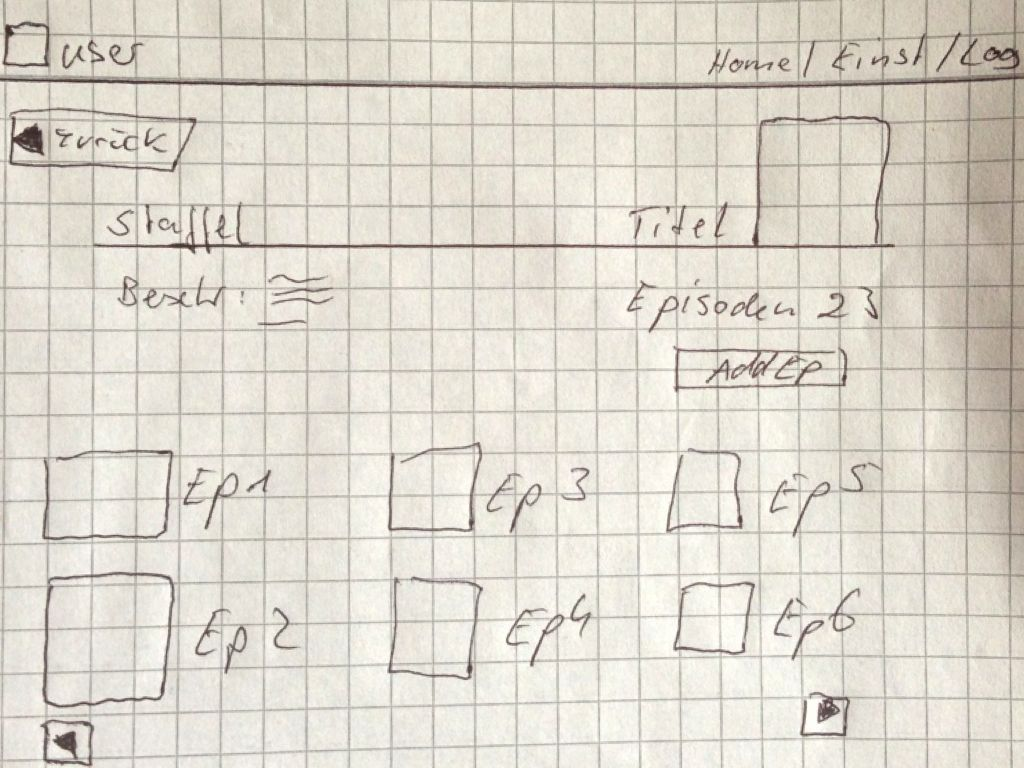
\includegraphics[width=.5\textwidth]{../images/dokulayout/staffel.jpg}}
\hfill % alternativ auch \hspace{1cm} für genaue Angaben
\subfloat[Episode anlegen \label{pic:episodeanlegen}]{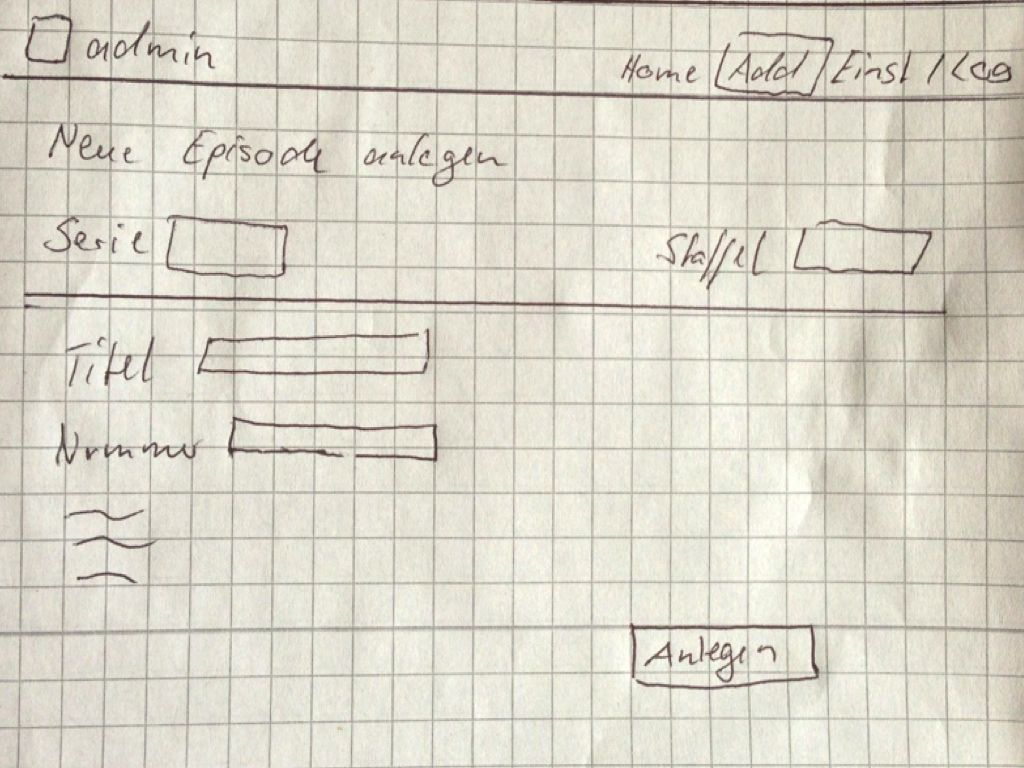
\includegraphics[width=.5\textwidth]{../images/dokulayout/anlegen.jpg}}
\hfill %
\caption{GUI Layout Skizzen: Seasonübersicht und Verwaltung }
\label{gui-skizzen-season-verwaltung}
\end{figure}

Bei der Planung der GUI, wurden die einzelnen Seiten nach entsprechenden Ideen konzipiert und weiterentwickelt. Die vorgestellten Entwürfe sollten einen kurzen Einblick in die Planungsphase geben und dienten in dieser Form keiner finalen Vorlage, nach der die Entwicklung stattfindet. Aus diesem Grund wird hier im weiteren nicht auf jede einzelne Unterseite eingegangen.\\ Während bei den ersten Varianten vorallem der mögliche Aufbau und die Darstellung der einzelnen Elemente im Vordergrund stand, wurden in späteren Versionen speziell auf entsprechende Funktionalität und Verweisen geachtet. Dabei entstand unter anderem die Adminansicht, welche die Kategorien um verwaltende Optionen erweitert. Ob jede Vorstellung realisierbar bzw. im Projektkontext notwendig ist und wie sich entsprechendes Layout letztendlich entwickelt hat, wird in der Umsetzung dargestellt.\\

\newpage
\subsection{Umsetzung}

Da im Voraus schon auf eine ordentliche Projektstruktur und dementsprechend wiederverwertbare Klassen gesetzt vorhanden waren, konnten diese für den User-Client wieder genutzt werden.\\

Für die GUI sollte \textit{Swing} verwendet werden, welches standardmäßig bei der Komponentenpositionierung auf fixe Pixel setzt. Als Alternative stand ein GUI Builder im Raum oder ein ordnentlicher Layoutmanager.\\
Die Wahl fiel dabei auf den Layout Manager namens MigLayout\footnote{\url{http://www.miglayout.com/}}.\\

Das Ziel für den User-Client war in erster Linie die Basisfunktionen verfügbar zu machen. In Bezug auf zuvor erstellte Konzeptskizze, zeigte sich, dass viele Funktionen angedacht wurden, die für die letztendliche Realisierung keine bedeutende Rolle spiele und aus diesem Grund ersetz wurden. Die gesamte Home Seite stellt nun eine funktionale Übersicht über vorhandene Serien dar. Eine Auswahl führt zu einer kurzen Vorschau, die in der Detailansicht dann die Informationen einer Serien mit Staffeln und Episodenvorschau hervorruft. Alle Funktionen wie Listenerstellung oder Übersicht, sowie Episodendetails konnten aus zeitlichen Gründe nicht mehr umgesetzt werden. Dadurch ergaben sich nun bei Abgabe folgende Funktionen, die anhand von GUIScreenshots einen Einblick in die Umsetzung geben sollen:

\begin{itemize}
  \item Registrierung eines neuen Accounts über XMPP und REST API
  \item Anmeldung via XMPP und REST API
  \item Auslesen der Benutzerdaten über REST API
  \item Auslesen von Serien über REST API
  \item Auslesen von Staffeln über REST API
  \item Auslesen von Episoden über REST API
  \item Anlegen einer neuen Serie über REST API
  \item Abonnieren einer Serie über XMPP PubSub Extension
  \item Empfangen von Notifcations über XMPP PubSub Extension
\end{itemize}



\begin{figure}[H]
  \centering
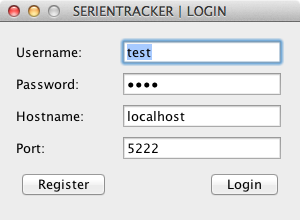
\includegraphics[width=0.5\textwidth]{../images/screenshots/client-login.png}
\caption{Anmeldung via XMPP und REST API}
\label{login}
\end{figure}

\begin{figure}[H]
  \centering
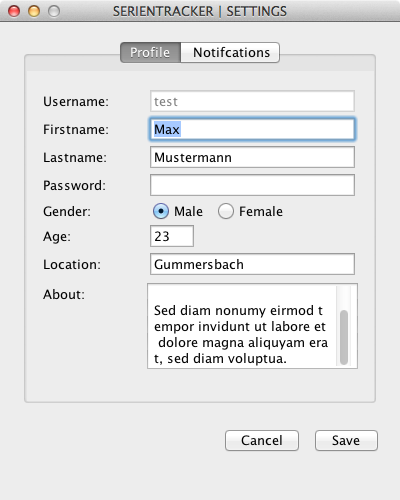
\includegraphics[width=0.5\textwidth]{../images/screenshots/client-user-settings.png}
\caption{Auslesen der Benutzerdaten über REST API}
\label{settings}
\end{figure}

 \begin{figure}[H]
   \centering
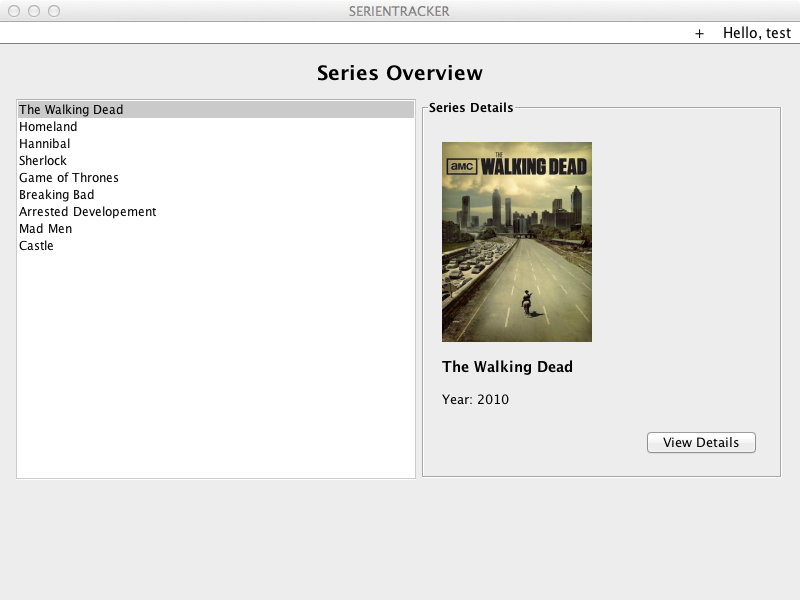
\includegraphics[width=0.7\textwidth]{../images/screenshots/client-series-overview.png}
\caption{Auslesen von Serien über REST API}
\label{overview}
\end{figure}

\begin{figure}[H]
  \centering
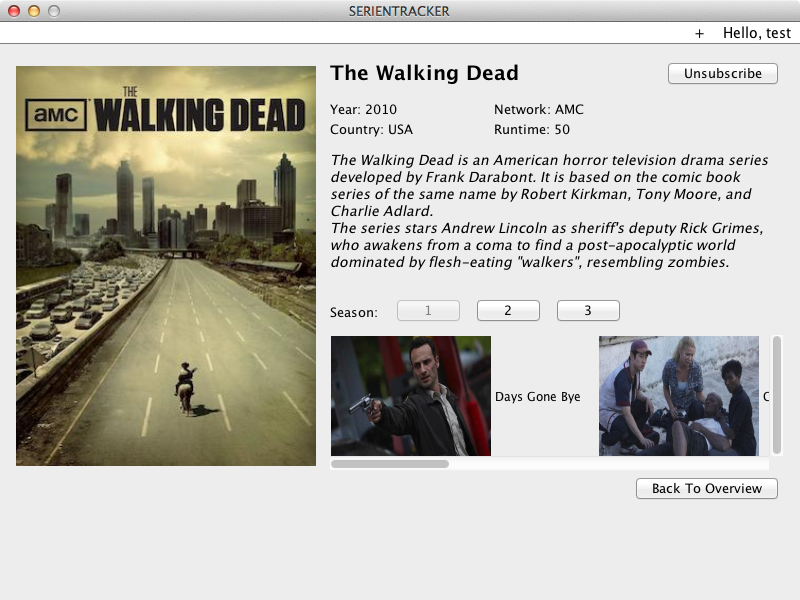
\includegraphics[width=0.7\textwidth]{../images/screenshots/client-series-details.png}
\caption{Auslesen von Staffeln und Episoden über REST API}
\label{details}
\end{figure}

\begin{figure}[H]
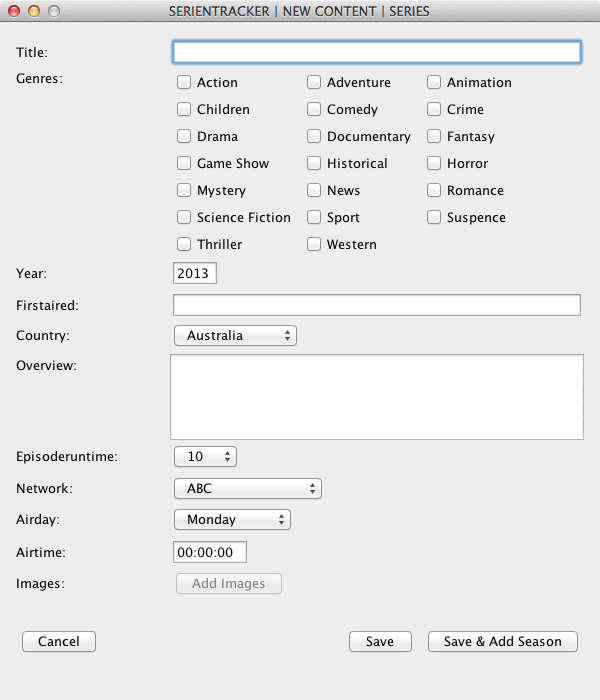
\includegraphics[width=1\textwidth]{../images/screenshots/client-new-content.png}
\caption{Anlegen einer neuen Serie über REST API}
\label{newcontent}
\end{figure}

\begin{figure}[H]
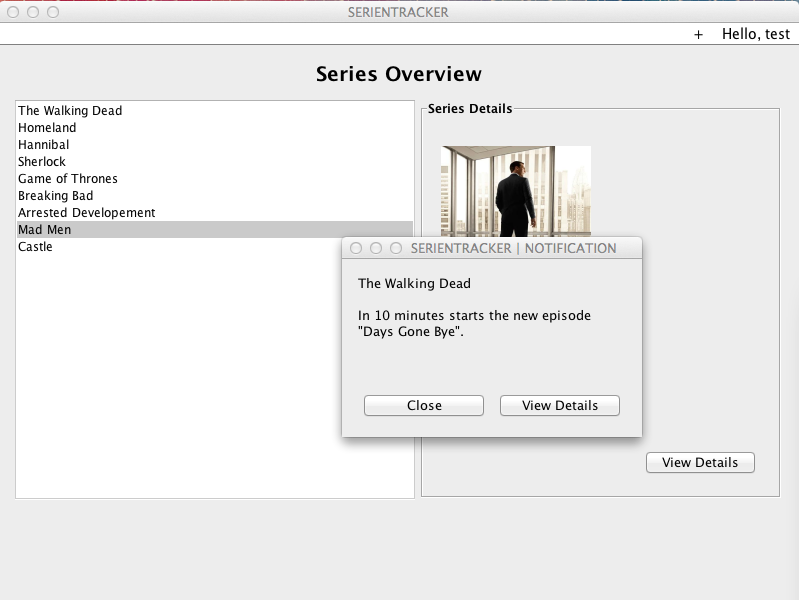
\includegraphics[width=1\textwidth]{../images/screenshots/client-notification.png}
\caption{Empfangen von Notifcations über XMPP PubSub Extension}
\label{notification}
\end{figure}

\newpage

\subsubsection{Übersicht Packages}

Zum Schluss eine Übersicht der nun vorhanden Packages und deren Funktionen im Zusammenhang mit dem User-Client.


\textbf{de.fhkoeln.gm.serientracker.client}\\
In diesem Paket befindet sich die Main-Klasse für den User-Client.

\textbf{de.fhkoeln.gm.serientracker.client.gui}\\
In diesem Paket befinden sich die Klassen für die Realisierung der GUI für den User-Client.

\textbf{de.fhkoeln.gm.serientracker.client.utils}\\
In diesem Paket befinden sich die mehrer modulare Klassen, die Aufgaben, wie Login, Subscription oder Session-Verwaltung übernehmen.

\textbf{de.fhkoeln.gm.serientracker.jaxb}\\
In diesem Paket befinden sich vom JAXB Generator generierten Objekte.

\textbf{de.fhkoeln.gm.serientracker.utils}\\
In diesem Paket befinden sich zwei Helfer-Klassen, zum einem der Hasher, zum Generieren eines MD5 Hashs sowie der Logger.

\textbf{de.fhkoeln.gm.serientracker.webservice}\\
In diesem Paket befindet sich die Main-Klasse für den REST Server, sowie die Klasse für die Servereinstellungen.

\textbf{de.fhkoeln.gm.serientracker.webservice.data}\\
In diesem Paket befinden sich die Data-Handler für die Ressourcen. Aufgrund des modularen Aufbaus wurden diese aus den Service-Klassen extrahiert. Sie sind das Bindeglied zwischen dem Service und dem File-Handler, siehe utils Paket.

\textbf{de.fhkoeln.gm.serientracker.webservice.resources}\\
In diesem Paket befinden sich die Services für die Ressourcen auf welche über die Clienten zugegriffen wird.

\textbf{de.fhkoeln.gm.serientracker.webservice.utils}\\
In diesem Paket befindt sich eine Helfer-Klasse, dem File-Handler, welche die Verbindung zwischen Dateisystem und JAXB Objekt implementiert.

\textbf{de.fhkoeln.gm.serientracker.xmpp}\\
In diesem Paket befindet sich die Main-Klasse für den XMPP-Debug-Client, sowie die Klasse für die Servereinstellungen.

\textbf{de.fhkoeln.gm.serientracker.xmpp.gui}\\
In diesem Paket befinden sich die Klassen für die Realisierung der GUI für den XMPP-Debug-Client.

\textbf{de.fhkoeln.gm.serientracker.xmpp.utils}\\
In diesem Paket befinden sich die mehrer modulare Klassen, die Aufgaben, wie Verbindungsaufbau oder Subscription-Verwaltung übernehmen.

\textbf{de.fhkoeln.gm.serientracker.bot}\\
In diesem Paket befindet sich die Main-Klasse für den Bot-Client. Siehe hierfür Abschnitt "Zusatz: Bot-Client".

\textbf{de.fhkoeln.gm.serientracker.bot.jobs}\\
In diesem Paket befinden sich die Klassen, die die Jobs übernehmen, wenn der Cronjob das Event ausführt.

\textbf{de.fhkoeln.gm.serientracker.bot.utils}\\
In diesem Paket befindt sich eine Wrapper-Klasse, welche die Verbindung zwischen der Quartz Scheduler API und dem Clienten implementiert.

\newpage

\subsection{Zusatz: Bot-Client}

Für das Veröffentlichen von Items, also den Notifications mit der Info über die bevorstehende Episodenaustrahlung, wurde ein Bot Client angelegt.\\
Der Bot-Client übernimmt dabei die Aufgabe pro Serie die Nodes anzulegen. Dazu scannt er die Datenbestand und wird zur jeder Serie drei Nodes anlegen, da ein User selbst entscheiden kann, ob er 5, 10 oder 15 Minute vorher informiert werden möchte. Die Node ID ist dabei im Format \textsf{series:\{Serien ID\}:\{[5|10|15]\}} definiert.\\
Gleichzeitig scannt er den Datenbestand nach den Episoden ab und prüft ob das Austrahlungsdatum in der Zukunft liegt.\\
Liegt es in der Zukunft wird ein Event angelegt. Dazu wurde die Quartz Scheduler Bibliothek\footnote{\url{http://quartz-scheduler.org}} eingesetzt. Mit ihr ist es möglich sogenannte Cronjobs anzulegen. Die beiden entwickleten Jobs \textit{ProfilerJob} und \textit{NotificationJob} übernehmen dabei die Verarbeitung.\\

Aus zeitlichen Gründen konnte  das Senden der automatisieren Notifcations nicht mehr implementiert werden. Zum Testen der Notifcation kann deshalb der XMPP Debug Client genutzt werden.
